\documentclass[12pt,a4paper]{report}
\usepackage{graphicx}
\usepackage{xcolor}
\usepackage{blindtext}
\usepackage{amsmath}
\graphicspath{ {./graficos-tp1/} }
\usepackage{fancyhdr}
\usepackage{amsmath}
% !TeX spellcheck = es
\usepackage[utf8]{inputenc}
\usepackage[spanish]{babel}

\makeatletter
\def\@makechapterhead#1{%
  %%%%\vspace*{50\p@}% %%% removed!
  {\parindent \z@ \raggedright \normalfont
    \ifnum \c@secnumdepth >\m@ne
        \huge\bfseries \@chapapp\space \thechapter
        \par\nobreak
        \vskip 10\p@
    \fi
    \interlinepenalty\@M
    \Huge \bfseries #1\par\nobreak
    \vskip 40\p@
  }}
\def\@makeschapterhead#1{%
  %%%%%\vspace*{50\p@}% %%% removed!
  {\parindent \z@ \raggedright
    \normalfont
    \interlinepenalty\@M
    \Huge \bfseries  #1\par\nobreak
    \vskip 40\p@
  }}
\makeatother

\begin{document}
\begin{titlepage}
	\pagestyle{fancy}
	\centering
			\textcolor{red}{\rule{15cm}{0.2mm}}\par \vspace{0.5cm}
	
\includegraphics[width=0.15\textwidth]{utn}\par
		\textcolor{red}{\rule{15cm}{0.2mm}}
		\par\vspace{1cm}

	{\scshape\LARGE Universidad Tecnológica Nacional\\Regional Buenos Aires \par}
	\vspace{1cm}
	{\scshape\Large Electrónica Aplicada II\par}
	\vspace{1cm}
	{\huge\bfseries Proyecto Integrador: Amplificador de Audio de Baja Potencia\par}
	\vspace{1cm}
	\begin{flushleft}
	Grupo N$^{\circ} 1$ - Curso: R4053\\ \vspace{0.1cm}
	\begin{tabular}{ |c|c| } 
	 \hline
	 Alumno &  Legajo\\
	\hline
	 Lucas Manuel Carra &  152624-8\\
	 \hline
	 Alessandro Ghezzo &  159281-6\\
	 \hline
	\end{tabular}
	\vspace{2cm}
	\vfill
	Docentes\par
	Ing.~Gustavo Randazo\\
	Ing.~Eduardo Jose Marchionni\\
	\end{flushleft}
	\textcolor{red}{\rule{15cm}{0.2mm}}

\end{titlepage}
\tableofcontents
\vfill
\textcolor{red}{\rule{15cm}{0.2mm}}\par \vspace{0.5cm}
\begin{flushleft}
\chapter{Introduccion}
\section{Consignas}
\subsection{Generales}
- Consignas generales a cumplir para todos los grupos de laboratorio: \par
\hspace{0.2cm} $ \bullet $ Todos los amplificadores en su diseño deben cumplir con las siguientes exigencias: \\
\hspace{1cm}   $ \bullet $ THD  $ \leq \% $ 1 \\
\hspace{1cm}   $ \bullet $ Fcif $ \geq $ 20 Hz \\
\hspace{1cm}   $ \bullet $ Fcsf $ \geq $ 20 KHz \\
\hspace{1cm}   $ \bullet $ Riaf $ \geq $ 80 K $ \Omega $ \\
- Cada grupo de trabajo deberá armar y probar el amplificador de audio según se le solicite en la consigna respectiva y simular tanto el equipo que arme como el “recíproco” que le toque, en lo que respecta a su etapa de salida. 
\\ Por ejemplo: si el amplificador para armar tiene una etapa de salida bipolar, el informe debe contemplar la simulación tanto del que armó, como el de una etapa de salida con MOS de enriquecimiento. Además, en dicho informe, debe haber una tabla  comparativa de los datos obtenidos, tanto medidos, como simulados. \\
\vspace{0.1cm}
\subsection{Particulares}
\hspace{0.2cm}   - Datos para el armado y puesta a punto del amplificador de audio: \\
\hspace{1cm}   $ \bullet $ Po = 10W \\
\hspace{1cm}   $ \bullet $ Se = 200mV \\
\hspace{1cm}   $ \bullet $ Tamb = 40 ºC \\
\vfill
\textcolor{red}{\rule{15cm}{0.2mm}}\par \vspace{0.5cm}
\newpage
\hspace{1cm}   $ \bullet $ RL =  8 $ \Omega $. \\
\hspace{1cm}   $ \bullet $ Con entrada NORMAL  y  ETAPA DE SALIDA MOSFET. \\
\hspace{0.2cm}   $ \bullet $ Informe del TP INTEGRADOR con simulaciones del circuito con salida MOS  y con salida BIPOLAR como se aclara en párrafos precedentes.   
\section{Objetivo}
$ \bullet $ Obtener algunos datos para observar semejanzas y  diferencias en los resultados previstos y otros datos de interés. 

$ \bullet $ Verificar la teoría y cálculos con las simulaciones.

\vfill
\textcolor{red}{\rule{15cm}{0.2mm}}\par \vspace{0.5cm}
\newpage
\chapter{Diseño del Amplificador}

\section{Descripción}
- Nuestro diseño se basa en 3 etapas y realimentación negativa: \\
\hspace{1cm}   $ \bullet $ Etapa de Pre-excitadora (Pre amplifier)\\
\hspace{1cm}   $ \bullet $ Etapa Amplificadora (Driver)\\
\hspace{1cm}   $ \bullet $ Etapa de Salida (Power)\\
\hspace{1cm}   $ \bullet $ Realimentación (Feedback)\\
\begin{center}
$\boxed { 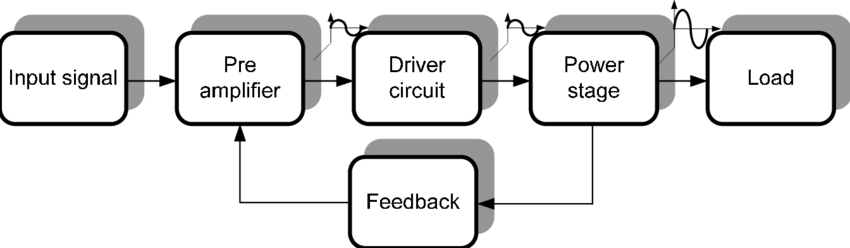
\includegraphics[width=0.5\textwidth]{DiagramaEnBloque} }$\\
\textit{Diagrama en bloque}
\end{center}
\vfill
\textcolor{red}{\rule{15cm}{0.2mm}}\par \vspace{0.5cm}
\newpage
\section{Etapa de Salida}
- Comenzamos nuestro diseño pensando en la etapa de salida, siendo esta la más importante en términos de potencia que maneja y disipación de energía. \\
- El requerimiento en el que nos basamos será la potencia a la cual someteremos al parlante del amplificador, representado por una resistencia de carga de 8 $ \Omega $. \\
- Elegimos una de transistores complementarios en modo colector común para que cada uno opere sobre medio ciclo de la señal de entrada, de esta manera mantenemos el consumo estático nulo (o muy bajo dependiendo de si utilizamos clase B o AB - se explicará más adelante en el proyecto) y generamos una ganancia de corriente sobre la carga para llegar a la potencia requerida.

\begin{center}
$\boxed { 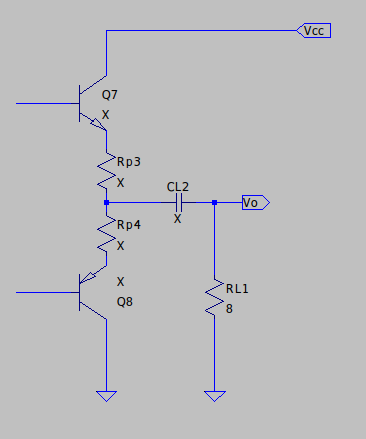
\includegraphics[width=0.355\textwidth]{EtapaSalidaTBJ} }$
$\boxed { 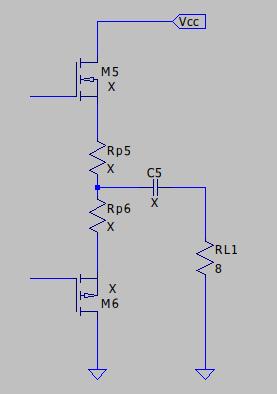
\includegraphics[width=0.3\textwidth]{GenericMosSalida} }$\par
\textit{Etapas de Salida TBJ y MOS}
\end{center}

\vfill
\textcolor{red}{\rule{15cm}{0.2mm}}\par \vspace{0.5cm}
\newpage
\subsection{Calculo de la Tensión y Corriente de Salida Máxima}

- Nuestro requerimiento de Potencia de salida es de 10 W.\\
- Utilizamos esto para calcular la tensión de salida máxima y la fuente que vamos a necesitar.\\ \vspace{0.2cm}

\subsubsection{Par de Transistor Bipolar de Juntura}

$ Po = \frac{Vo_{ef}^2}{R_L} = 10$ \\ \vspace{0.2cm}
$ Vo_{ef} = \frac{Vo_{max}}{\sqrt[2]{2}} $ \\ \vspace{0.2cm}
$ Vo_{max} = \sqrt[2]{P_o \times R_L \times 2} = 12.65 V $ \\ \vspace{0.2cm}
$ Io_{max} = \frac{12.65}{8} = 1.58 A $ \\ \vspace{0.2cm}

Para el calculo de la tensión de la fuente consideramos un semi-ciclo de la señal donde Q1 conduce y Q2 está al corte:\\
\begin{center}
$\boxed { 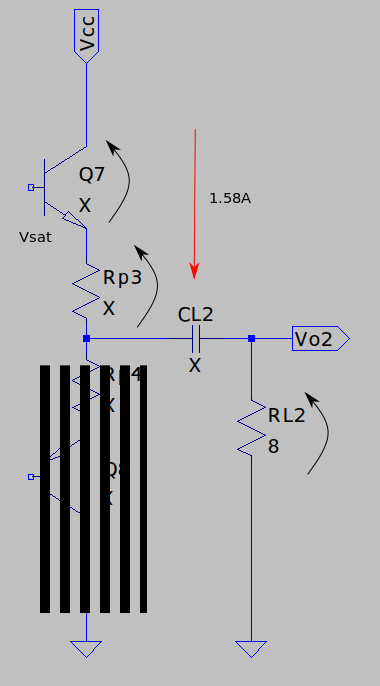
\includegraphics[width=0.3\textwidth]{SalidaTBJCalculoVCC} }$ \\
\vspace{0.2cm}
$\boxed { Vcc = 2 \times V+ = 2 \times (1.58A \times (8 + 0.39 ) + V_{sat} ) =  30.5} $ \\

Finalmente adoptamos una fuente de 35 V como factor de seguridad y por ser un valor más tipico.

\end{center}
$V_{sat} = 2.0 \hspace{0.1cm} Vdc_{(MAX)} \hspace{0.2cm} @ I_C = 3 A_{DC} $ \\


\vfill
\textcolor{red}{\rule{15cm}{0.2mm}}\par \vspace{0.5cm}
\newpage

\subsubsection{Par de Transistor MOSFET}

- Para la salida MOSFET el cálculo es similar: \\
- La $V_{omax} $ y $I_{omax} $ coinciden con nuestro planteo anterior. \\
- El mismo caso para las resistencias de protección térmica. \\
- La alimentación debería modificarse dado el planteo debajo pero mantendremos la fuente de 35V para mantener un solo diseño apto para ambas salidas.\\
$\boxed { Vcc = 2 \times V+ = 2 \times (1.58A \times (8 + 0.39 ) + V{DS_{ON}} ) =  13.21 \times 2 = 26.4V } $ \\

\vfill
\textcolor{red}{\rule{15cm}{0.2mm}}\par \vspace{0.5cm}
\newpage

\subsection{Calculo de las Resistencias de Protección térmica}
- Las resistencias a ambos lados de los transistores de salida son Termistores del tipo PTC (Positivite temperature coefficient$^1 $ ), que van a aumentar su impedancia a medida que la temperatura aumente para mantener la corriente constante.\\
\vspace{0.2cm}
- Se calculan como:\\
\hspace{0.5cm} $\bullet Rp_{max}$ es un 10\% de la carga.\\
\hspace{0.5cm} $\bullet Rp_{min}$ es un 5\% de la carga.\\
\vspace{0.4cm}
$ \boxed{ 0.4 < Rp < 0.8 } $ \\
\vspace{0.4cm}
El valor comercial más proximo es 0.39 - Es aceptable.
\begin{center}
$ \boxed{ Rp1 = Rp2 = 0.39 } $ \\
\end{center}

\subsubsection{Potencia disipada}

La potencia que van a disipar va a ser de:
\begin{center}
$ \boxed{(\frac{Io_{max}}{2})^2 \times Rp = 0.48W } $ \\
Comercial 20\% - 1 W
\end{center}

1 - Termistores PTC - https://en.wikipedia.org/wiki/Thermistor

\vfill
\textcolor{red}{\rule{15cm}{0.2mm}}\par \vspace{0.5cm}
\newpage

\subsection{Elección de los transistores}
\subsubsection{Par de Transistor Bipolar de Juntura}
Elejimos los transistores de salida teniendo en cuenta 4 factores: \\ \vspace{0.2cm}
\hspace{1cm}	$ \bullet Ic_{max} > 1.6A $\\ \vspace{0.2cm}
\hspace{1cm}	$ \bullet BV_{ceo} > \frac{35V}{0.75} = 46.66V $\\ \vspace{0.2cm}
\hspace{1cm}	$ \bullet Pdav_{max}  >  \frac{(1.1 * V_{cc})^2}{40 * 0.8 R_L} = 3.975W $\\ \vspace{0.2cm}
\hspace{1cm}	$ \bullet hFE - El mas alto $\\ 
\vspace{1cm}

\begin{center}
\begin{tabular}{ |c|c|c|c|c| } 
\hline
Transistor & Icmax & BVceo & Pdavmax & hFE \\
\hline
BDW93/94C & 12A  & 100V & 80W & 1000 \\
\hline
TIP102/107 & 8A & 100V & 80W & 1000\\
\hline
TIP122/127 & 5A & 100V & 65W & 1000 \\
\hline
\end{tabular}
\end{center}
\vspace{0.2cm}

$ \bullet $  Esta tabla corresponde a los transistores que electrocomponentes dispone publicados y, debido a la falta de stock del BDW93C y del TIP107, elegimos los transistores TIP122 y TIP 127 como par complementario de la etapa de salida\\
$ \bullet $  El par complementario TIP 122 / TIP 127 de tipo D'Arlington cumple todos nuestros requerimientos y nos da un hFE alto.\\


\subsubsection{Par de Transistor MOSFET}
- Aplicamos los mismos criterios que la selección de TBJ pero con sus parámetros análogos.\\
\hspace{1cm} - $ BV_{VDS} > \frac{Vomax}{0.75} = 16.86V $\\
\hspace{1cm} - $ I_{D_{MAX}} \geq 2A  $\\
\hspace{1cm} - $ Pd_{MAX} > \frac{(1.1 \times Vcc)^2}{40\times 0.8 \times 8\Omega} > 4.25W  $\\
- Elegimos el par de transistores MOS de potencia IRFP240/IRFP9240 por su disponibilidad en el mercado y porque satisface nuestros requerimientos.\\
\hspace{1cm} - $ BV_{VDS} \simeq 200V $\\
\hspace{1cm} - $ I_{D_{MAX}} \simeq 18A  $ | $40^{\circ} $ C \\
\hspace{1cm} - $ Pd_{MAX} \simeq 150W  $ | $40^{\circ} $ C\\
\hspace{1cm} - $ g_{fs} = 6.9 [S] $\\
\hspace{1cm} - $ V_{DS_{ON}} = R_{DS_{ON}} \times I_{omax} = 284mV $\\
\
\hspace{1cm} - $ V_{GS_{ID=1.6A}} = 4.5V $ \\

\vfill
\textcolor{red}{\rule{15cm}{0.2mm}}\par \vspace{0.5cm}
\newpage
\subsection{Multiplicador de Tensión}
- El efecto de distorsión por cruce ocurre en los amplificadores de tipo B cuando al variar la señal de entrada se genera la transición de corte a la zona activa. Dado que el transistor que pasa de corte a activo tiene que superar su tensión de umbral $V_{SAT} $ sin una pre-polarización se produce el siguiente efecto que puede ser desagradable para el oido (como un zumbido):\\
\begin{center}
$ \boxed { 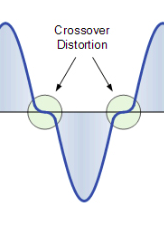
\includegraphics[width=0.3\textwidth]{Distorcionporcruce}   } $
\end{center}

- Para evitarlo, lo que hacemos es mantener una diferencia de potencial entre las bases de ambos transistores muy cercano a su 
$V_{SAT} $, de esta manera se subsanar el efecto a costo de un consumo de corriente estático relativamente bajo. \\
- Existen varias maneras de hacerlo, desde un resistor variable, varios diodos o el 'multiplicador' en base a un BJT, elegimos ir por este último.\\
- La leve polarización hace que denominemos al amplificador como clase AB.\\

\vfill
\textcolor{red}{\rule{15cm}{0.2mm}}\par \vspace{0.5cm}
\newpage

\begin{center}
$ \boxed { 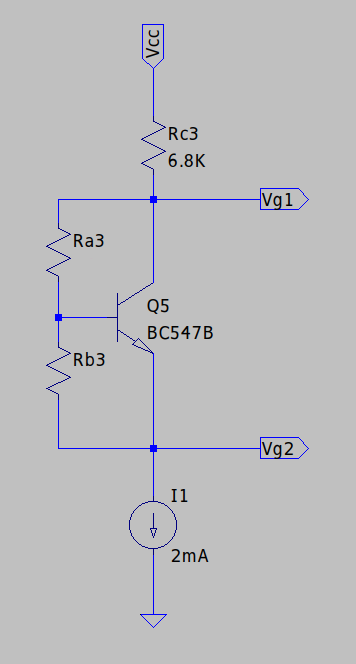
\includegraphics[width=0.3\textwidth]{MultiplierMOS}   } $
\end{center}

\subsubsection{Calculo}
- El multiplicador tiene una relación de: $ \Delta V = V_{BE} \times (1 + \frac{Ra}{Rb})$ \\
- Para el caso del MOSFET \\
- $ Vmult = 2 \times V_{GS} + 2 \times V_{rp} = 10.43V $ \\
- $ V_{oEST} = \frac{Vcc}{2} = 17.5 V $ \\
- $V_{mult-} = V_{oEST} - (V_{GS} + V_{RP2}) = 9.75V $ \\
- $V_{mult+} = V_{oEST} - (V_{GS} + V_{RP1}) = 20.25 V $ \\
- De nuevo asumimos una corriente de 2mA en la rama del multiplicador y ahora sabemos que la corriente Ig es = 0. \\
\begin{center}
$\boxed { 
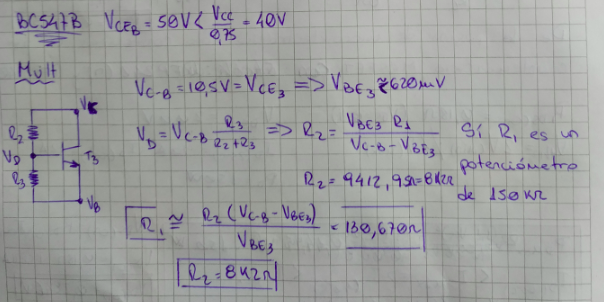
\includegraphics[width=0.7\textwidth]{MultiplicadorAMano} } $
\end{center}
- Para el circuito TBJ el planteo es similar, solo que la diferencia de tensión buscada para la prepolarización varía, en nuestro caso alrededor de los 2.5V.
\vfill
\textcolor{red}{\rule{15cm}{0.2mm}}\par \vspace{0.5cm}
\newpage

\subsection{Diseño Preliminar}
\subsubsection{TBJ}
\begin{center}
$\boxed { 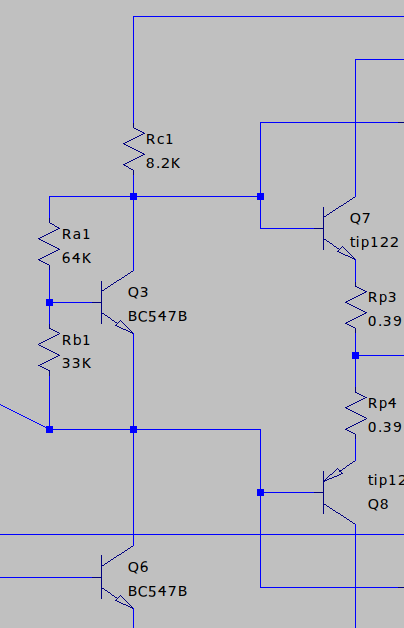
\includegraphics[width=0.5\textwidth]{EtapaSalidaFinalTBJ} }$ \\
\end{center}
El diseño final de la etapa de salida es el siguiente. \\ \vspace{0.2cm}
\hspace{1cm}	$ \bullet $ Par complementario NPN - PNP (Clase AB) \\
\hspace{1cm}	$ \bullet $ Multiplicador de tensión (Clase AB). \\
\hspace{1cm}	$ \bullet $ Termistores de protección termica. \\
\hspace{1cm}	$ \bullet $ Carga de 8 Ohm (Parlante) \\
- Nota: Más adelante en evaluacion térmica decidimos duplicar la etapa de salida para repartir la corriente entre ambos pares.

\subsubsection{MOSFET}
\begin{center}
$\boxed { 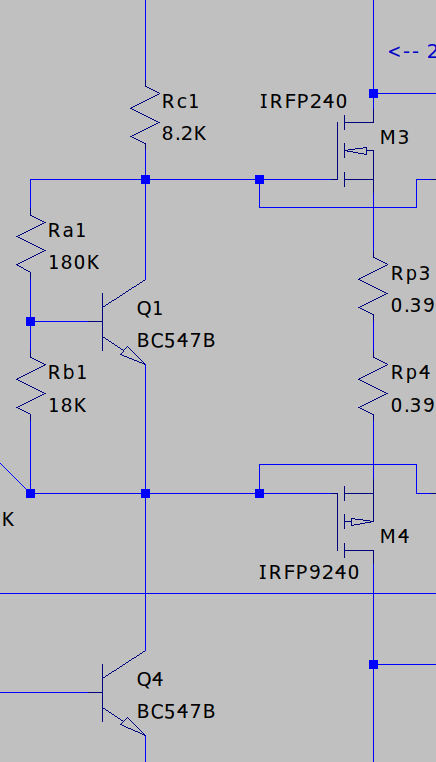
\includegraphics[width=0.5\textwidth]{EtapaSalidaMOS} }$ \\
\end{center}
El diseño final de la etapa de salida es el siguiente. \\ \vspace{0.2cm}
\hspace{1cm}	$ \bullet $ Par complementario NMOS - PMOS (Clase AB) \\
\hspace{1cm}	$ \bullet $ Multiplicador de tensión (Clase AB). \\
\hspace{1cm}	$ \bullet $ Termistores de protección termica. \\
\hspace{1cm}	$ \bullet $ Carga de 8 Ohm (Parlante) \\
- Nota: Más adelante en evaluacion térmica decidimos duplicar la etapa de salida para repartir la corriente entre ambos pares.

\vfill
\textcolor{red}{\rule{15cm}{0.2mm}}\par \vspace{0.5cm}
\newpage

\section{Etapa Amplificadora}
- El objetivo de esta etapa es tomar la señal ya pre-amplificada por la excitadora y llevarla al nivel de tensión final que vamos a necesitar en la salida. \\
- Elejimos una topología de tipo Emisor Común Degenerado (mejorado) para mantener la ganancia dependiente de la relación entre resistores y no de las variaciones características impredecibles del transistor, mejorando la distorsión (linealidad) y estabilidad a costo de ganancia.\\

\begin{center}
$\boxed { 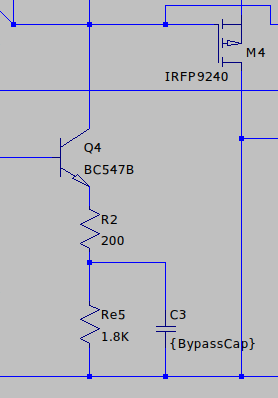
\includegraphics[width=0.5\textwidth]{EtapaAmplificadora} }$ \\
\end{center}

- Elegimos el BC547B más que nada por accesibilidad y $h_{FE} $ suficiente.\\
- Se planteo tener una corriente de alrededor de 2mA sobre esta rama.

\vfill
\textcolor{red}{\rule{15cm}{0.2mm}}\par \vspace{0.5cm}
\newpage
\section{Etapa Pre-excitadora}
- El objetivo de la etapa pre-excitadora normalmente es tomar la señal en tensiones muy bajas (máx 200mV por requerimiento inicial) y llevarlas a un nivel superior antes de pasarselo a la etapa amplificadora. \\
- Debe proveer una resistencia de entrada de al menos 80K. \\
- Elegimos una topología de tipo Emisor Común Degenerado que nos va a brindar una ganancia de tensión de entre 10 y 20 veces.

\begin{center}
$\boxed { 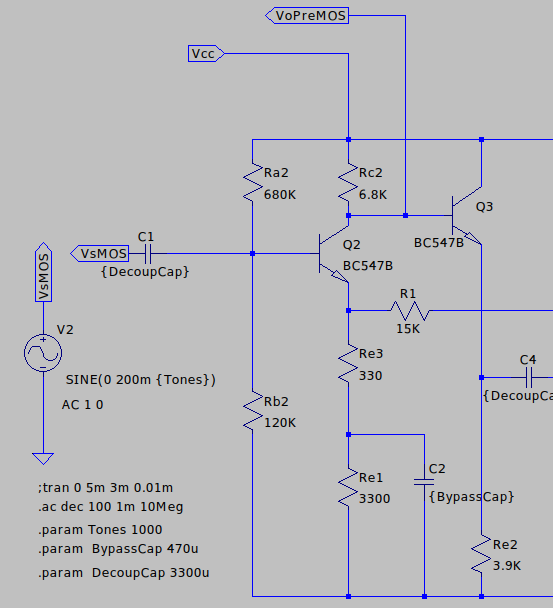
\includegraphics[width=0.5\textwidth]{EtapaEntrada} }$ \\
\end{center}

\section{Realimentación Negativa}
\subsection{Identificación General}
- Utilizaremos una realimentación de tipo Series-Shunt (Tensión-Serie), donde muestreamos la tensión de la salida y reinyectamos tensión a la entrada.\\
- El efecto de esta realimentación será:\\
\hspace{0.2cm} $\bullet $ Aumento de la resistencia de entrada por el factor de realimentación D.\\ \vspace{0.1cm}
\hspace{0.2cm} $\bullet $ Disminusión de la resistencia de salida por el factor de realimentación D.\\ \vspace{0.1cm}
\hspace{0.2cm} $\bullet $ Control de la ganancia del circuito a través de la malla B. \\ \vspace{0.1cm} 
\begin{center}
$\boxed { 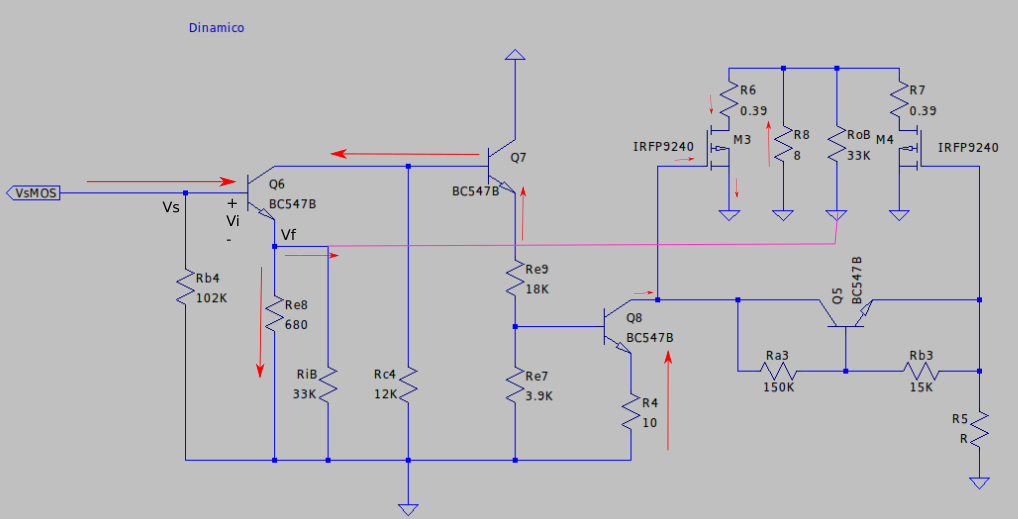
\includegraphics[width=1\textwidth]{AnalisisDeFase} }$ \\
\end{center}
- Corroboramos la realimentación negativa observando las fases en el circuito dinámico.
\vfill
\textcolor{red}{\rule{15cm}{0.2mm}}\par \vspace{0.5cm}
\newpage
\subsection{Malla Beta}
- Nuestra malla de realimentación B es un simple divisor resistivo conformado por la Rf y la Re de la entrada.
\begin{center}
$\boxed { 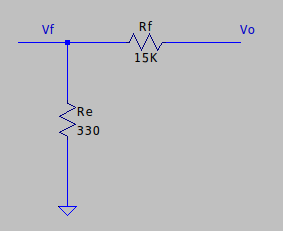
\includegraphics[width=0.6\textwidth]{MallaB} }$ \\
\end{center}
\[ \beta \simeq \frac{Vf}{Vo} = \frac{330}{330 + 15K} = 6.66e^{-5} \] \\
\[ Avsf \simeq 1 + \frac{330}{15K} = 46.45 \]

\vfill
\textcolor{red}{\rule{15cm}{0.2mm}}\par \vspace{0.5cm}
\newpage
\section{Diseño Final}
El resultado obtenido es el siguiente:
\begin{center}
$\boxed { 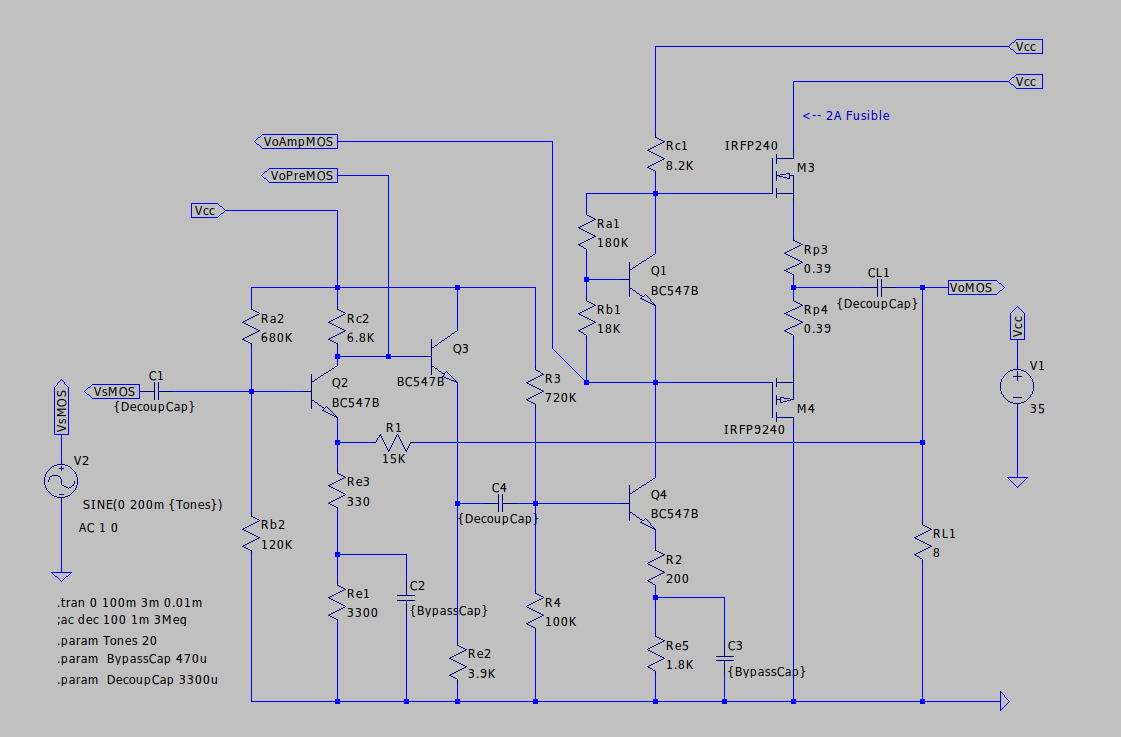
\includegraphics[width=1\textwidth]{DisenoFinalUlt} }$ \\
\end{center}
\vfill
\textcolor{red}{\rule{15cm}{0.2mm}}\par \vspace{0.5cm}
\newpage

\chapter{Simulación}
- Todos los gráficos presentados a continuación fueron capturado por el circuito de salida MOSFET, el comportamiento del equivalente TBJ es casi identico.

\subsection{Preamplifcación}
- Observamos la señal de la etapa pre amplificador con el circuito a lazo abierto. \\
- La señal experimenta una ganancia de tensión de 17.2 veces. \\ \vspace{0.2cm}

$ Avsim_{pre} = \frac{3.44V}{200mV} = 17.2 $ 

\begin{center}
$\boxed { 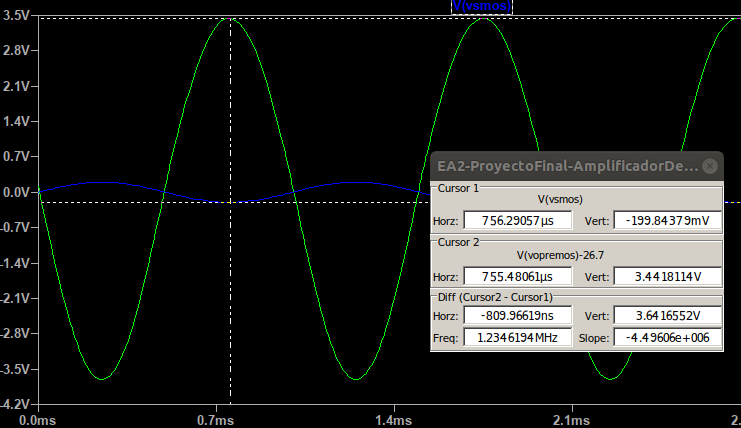
\includegraphics[width=1\textwidth]{VoPre} }$ \\
\end{center}
\textit{ {\tiny Nota: A todas las señales involucradas en la gráfica se les removió el nivel de continua para facilitar su visibilidad.} }
\vfill
\textcolor{red}{\rule{15cm}{0.2mm}}\par \vspace{0.5cm}
\newpage
\subsection{Amplificación}
- Observamos la señal de la etapa amplificadora teniendo en cuenta la realimentación para controlar su saturación. \\
- Tenemos una amplificación de tensión total de 52 veces. \\ \vspace{0.2cm}

\begin{center}
$\boxed { 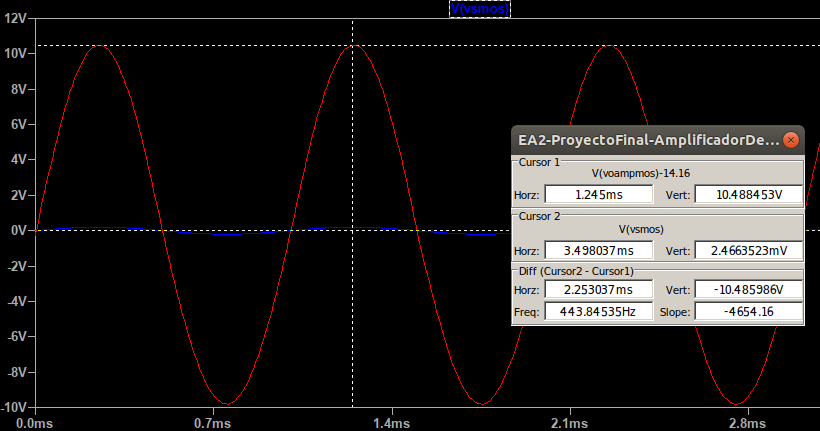
\includegraphics[width=1\textwidth]{VoAmpFinal} }$ \\
\end{center}
\textit{ {\tiny Nota: A todas las señales involucradas en la gráfica se les removió el nivel de continua para facilitar su visibilidad.} }
\vfill
\textcolor{red}{\rule{15cm}{0.2mm}}\par \vspace{0.5cm}
\newpage
\subsection{Salida}
- Observamos la señal de salida.\\
- Miramos tanto tensión como corriente. \\

\begin{center}
$\boxed { 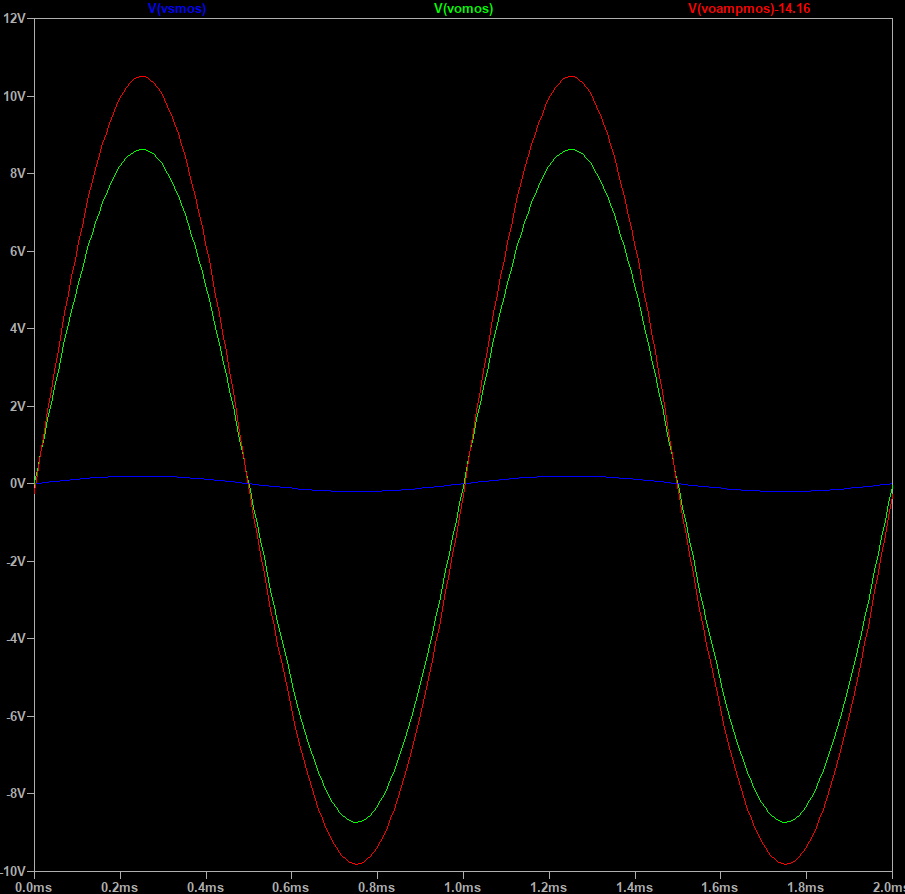
\includegraphics[width=1\textwidth]{VoFinal} }$ \\
Tension
\end{center}

\begin{center}
$\boxed { 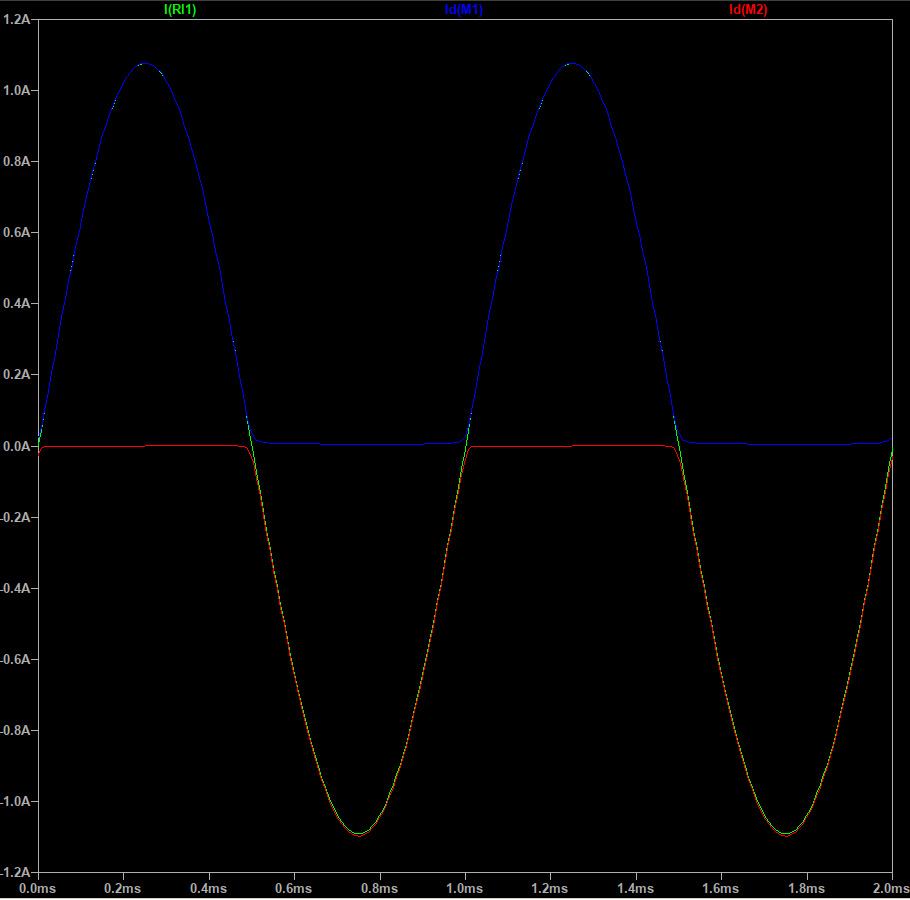
\includegraphics[width=1\textwidth]{CorrienteFinal} }$ \\
Corriente
\end{center}

- Tanto tensión como corriente se ven bastante bien, la distorsión por cruce es practicamente inexistente dada la leve polarización de los transistores durante su ciclo "contrario".\\
- La corriente de salida máxima observada es de 1.2A, relativamente cercana a nuestra primera proyección de 1.5A.\\

\begin{center}
$\boxed { 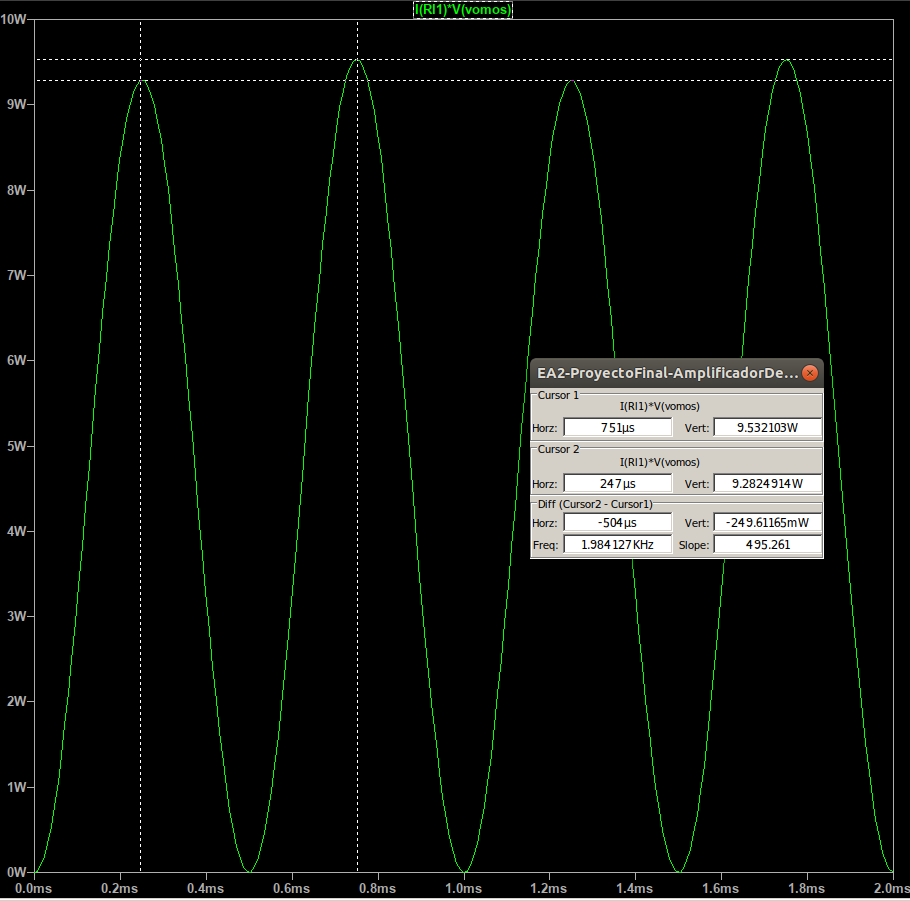
\includegraphics[width=1\textwidth]{PotenciaFinal} }$ \\
Potencia
\end{center}

- Nos encontramos dentro de el requerimiento de 10W +/- 1\%.

\vfill
\textcolor{red}{\rule{15cm}{0.2mm}}\par \vspace{0.5cm}
\newpage

\subsection{Distorsión Armónica}
La distorsión armonica se calcula a partir de: \\ \vspace{0.2cm}
\hspace{1cm} $\bullet $ La amplitud de la armonica fundamental \\ \vspace{0.2cm}
\hspace{1cm} $\bullet $ La amplitud de las amplitudes de las armonicas siguientes. \\ \vspace{0.2cm}

\[ THD = \frac{\sqrt[2]{\sum\limits_{i=2}^n V_{n-rms}^2}}{V_{fund-rms}}  \]

Tomamos la salida generada por una señal senoidal de 1Khz, y aplicandole la FFT observamos lo siguiente:

\begin{center}
$\boxed { 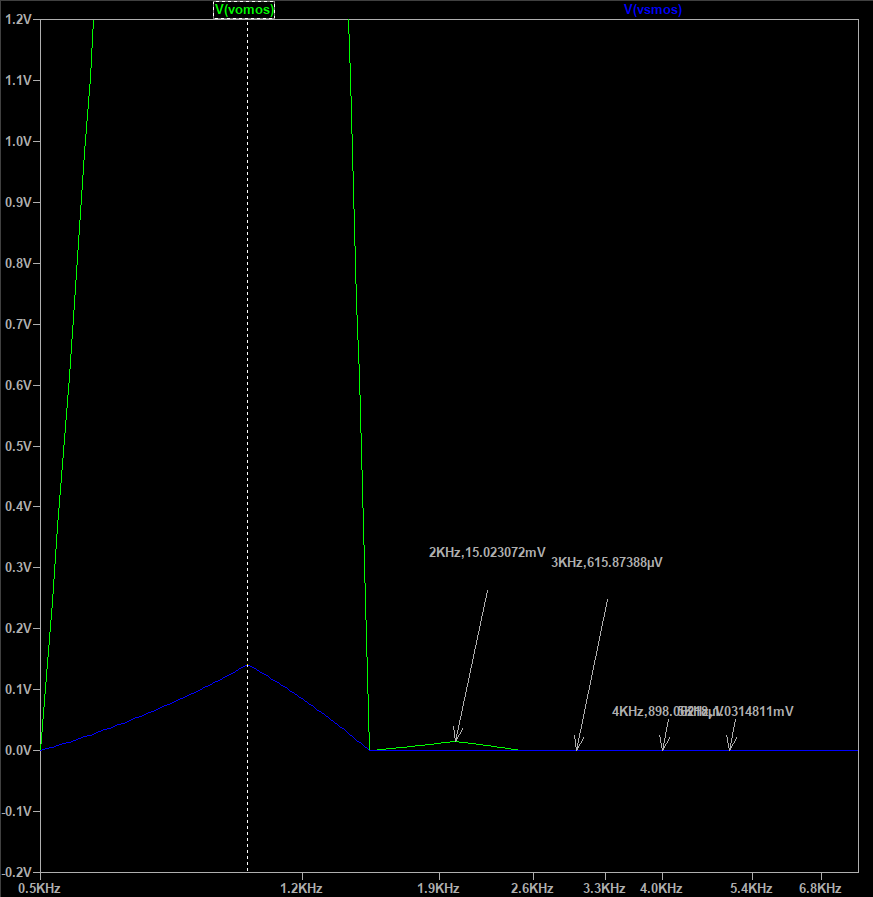
\includegraphics[width=0.75\textwidth]{Distorsion} }$ \\
\end{center}

\vfill
\textcolor{red}{\rule{15cm}{0.2mm}}\par \vspace{0.5cm}
\newpage
Nuestra armónica fundamental presenta una amplitud de 6.13V. \\
Y obtenemos pequeños picos de armonicas nuevas en:\\
\hspace{0.5cm} $\bullet $ 2KHz: 15mV \\ \vspace{0.2cm}
\hspace{0.5cm} $\bullet $ 3KHz: 617uV \\ \vspace{0.2cm}
\hspace{0.5cm} $\bullet $ 4KHz: 800uV \\ \vspace{0.2cm}
\hspace{0.5cm} $\bullet $ 5KHz: 1mV \\ \vspace{0.2cm}
Entonces:\\ \vspace{0.2cm}

\[ THD = \frac{\sqrt[2]{(15mV)^2 + (617uV)^2 + (800uV)^2 + (1mV)^2 }}{6.13V} = 0.00608 \]

Porcentualmente tenemos una distorción del 0.6\%, lo cuál está dentro de nuestro requerimiento de una THD menor o iguál al 1\%.

Si necesitasemos mejorarla, las maneras serían:\\ \vspace{0.2cm}
\hspace{0.5cm} $\bullet $ Reevaluar la distorsión por cruce en la etapa de salida variando la polarización de las bases para que se encuentren más cerca de la zona activa. \\ \vspace{0.2cm}
\hspace{0.5cm} $\bullet $ Investigar posibles no-linealidades en las etapas amplificadoras. \\ \vspace{0.2cm}
\hspace{0.5cm} $\bullet $ Aumentar la realimentación negativa. \\ \vspace{0.2cm}


\vfill
\textcolor{red}{\rule{15cm}{0.2mm}}\par \vspace{0.5cm}
\newpage

\subsection{Respuesta en frecuencia}
\begin{center}
$\boxed { 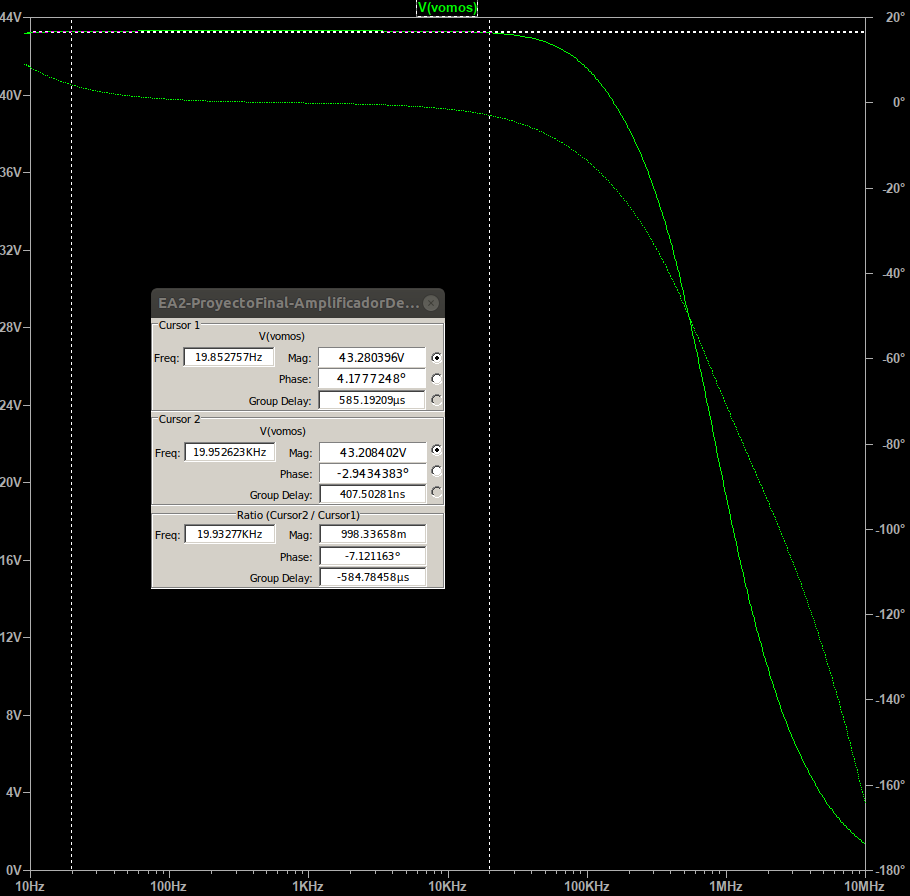
\includegraphics[width=0.75\textwidth]{RespEnFrecuencia} }$ \\
\end{center}

- Cumplimos los requerimientos de:\\
\hspace{0.2cm} $ \bullet $ Fci $\leq 20Hz $ \\ \vspace{0.1cm}
\hspace{0.2cm} $ \bullet $ Fcs $\geq 20KHz $ \\ \vspace{0.1cm}


\subsection{Resistencia de entrada}
\begin{center}
$\boxed { 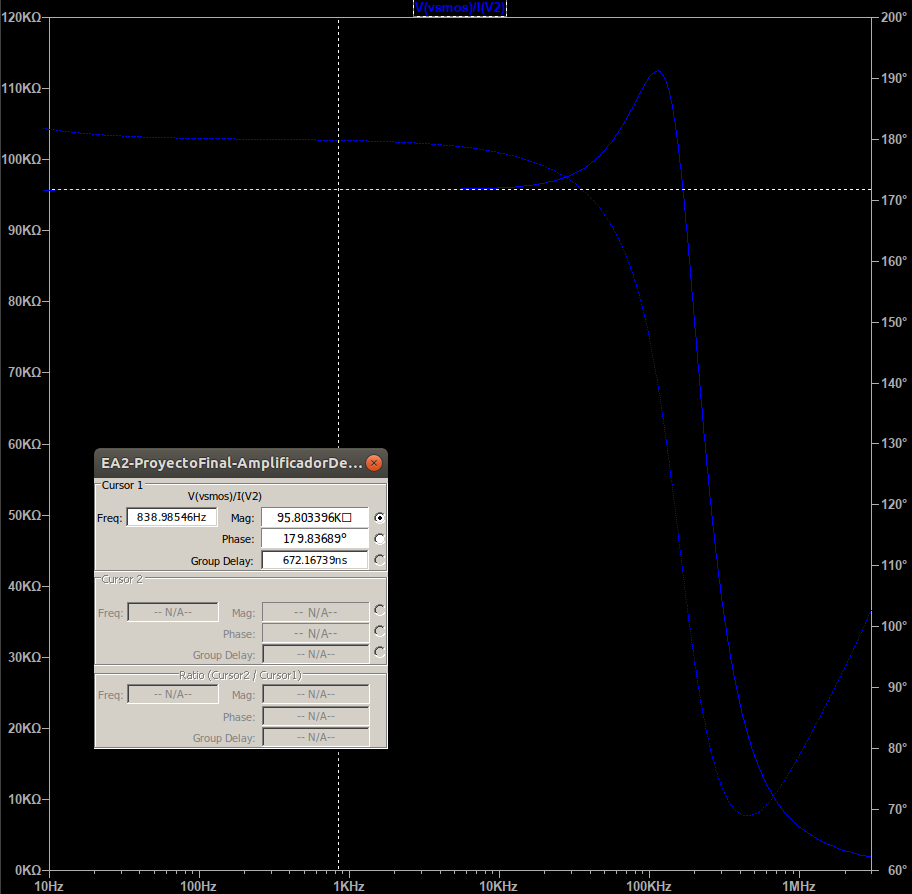
\includegraphics[width=0.75\textwidth]{Risf} }$ \\
\end{center}
Para el ancho de banda de operación observamos una resistencia de entrada de 95K $\Omega $, con lo cuál cumplimos el requerimiento de $Riaf \geq 80K\Omega $.

\chapter{Temperatura}
- Para la etapa de salida vamos a necesitar aplicar disipadores a los transistores dada su relativamente alta disipación y temperatura de operación. \\ \vspace{0.1cm}
- Consideramos el requisito inicial de temperatura normal de operación de $40^{\circ} $C. \\ \vspace{0.1cm}
- $ T = k * Tj - Ta $ \\
- Utilizamos un k de 0.5 para un diseño normal. 
$\boxed { 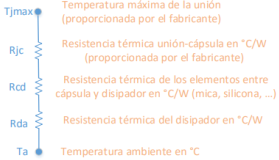
\includegraphics[width=0.7\textwidth]{Rth} }$ \\
$ Pd = 4.25 W $ \\ \vspace{0.1cm}
$ Pd = \frac{Tj - Ta}{Rth} = \frac{Tj - Ta}{Rcd + Rja + Rda}  $ \\ \vspace{0.1cm}
$ Rda = \frac{0.5 \times 150^{\circ}C - 40^{\circ}C}{4.25W}  
- 0.5 \frac{^{\circ}C}{W} - 0.83 \frac{^{\circ}C}{W} = 24.55 \frac{^{\circ}C}{W} = 6.91 \frac{^{\circ}C}{W} $\\ \vspace{0.1cm}
- Con estos valores de Rda podemos utilizar una gran variedad de disipadores en el mercado sin necesidad de paralelizar la etapa de salida.

\vfill
\textcolor{red}{\rule{15cm}{0.2mm}}\par \vspace{0.5cm}
\newpage

\chapter{Diseño CAD}
\subsection{Software}
- Elejimos KiCAD dado que es un software libre de automatización de diseño electrónico.

\subsection{Esquemático}
- Al diseño original agregamos:\\
-- Agujeros de montaje.\\
-- Conectores femeninos, masculinos y Jack para alimentación y señal, testing points, etc.\\
-- Dejamos espacio para colocar los disipadores de calor de la etapa de salida.
\begin{center}
$\boxed { 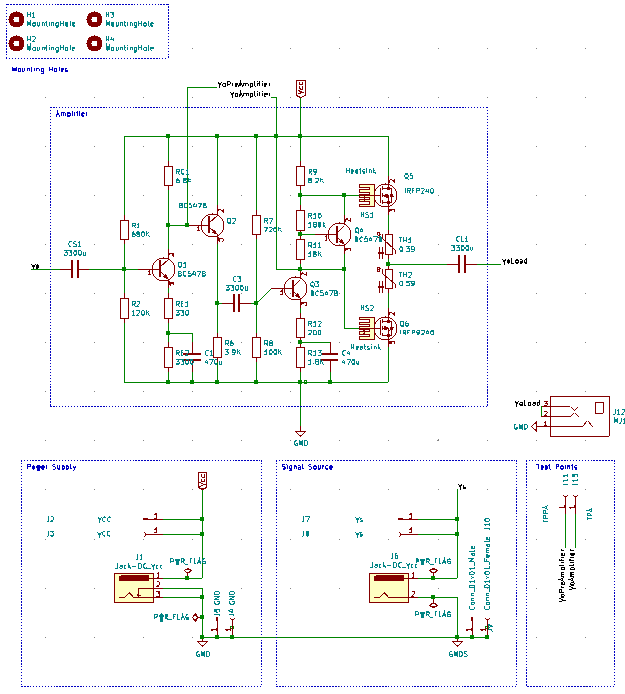
\includegraphics[width=0.6\textwidth]{Schematic} }$ \\
\end{center}
\vfill
\textcolor{red}{\rule{15cm}{0.2mm}}\par \vspace{0.5cm}
\newpage

\subsection{PCB}
- Posicionamos la fuente lo más cercano a la carga.\\
- Usamos un track-width mayor en las zonas de alta corriente.\\
- Un diseño de 2 capas es más que suficiente.\\
\begin{center}
$\boxed { 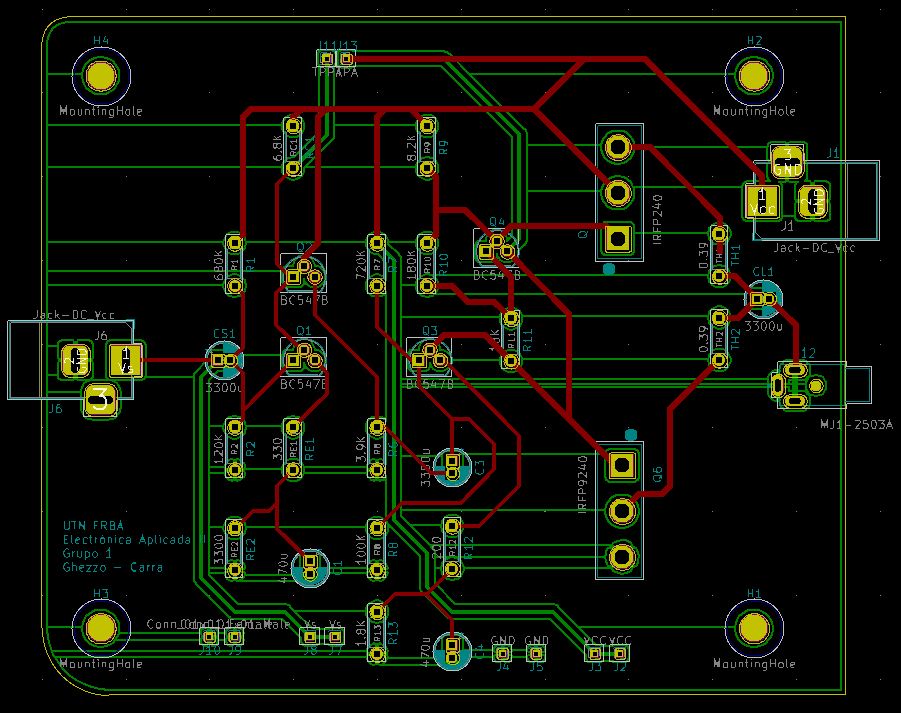
\includegraphics[width=1\textwidth]{KiCadComp} }$ \\
\end{center}
\vfill
\textcolor{red}{\rule{15cm}{0.2mm}}\par \vspace{0.5cm}
\newpage
\subsection{Render 3D}
\begin{center}
$\boxed { 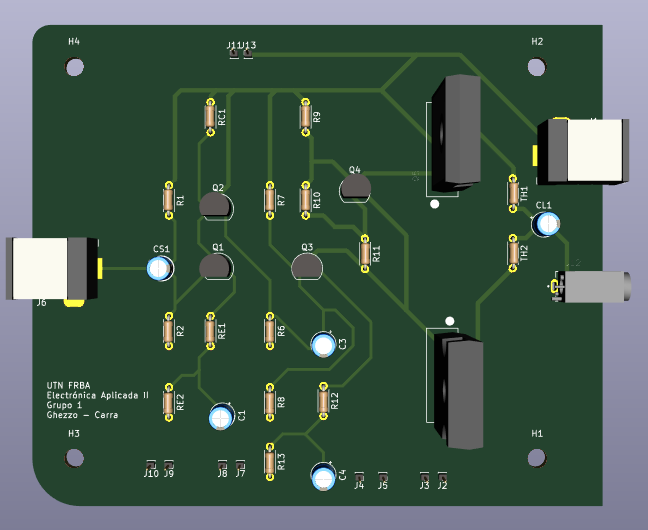
\includegraphics[width=1\textwidth]{Front3d} }$ \\
\end{center}
\begin{center}
$\boxed { 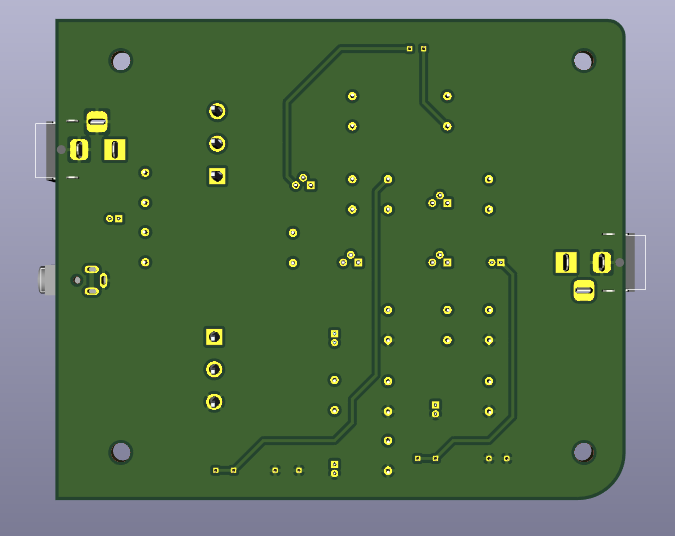
\includegraphics[width=1\textwidth]{Back3d} }$ \\
\end{center}
\vfill
\textcolor{red}{\rule{15cm}{0.2mm}}\par \vspace{0.5cm}
\newpage
\chapter{Bibliografía}
- Diseño De Amplificadores De Potencia De Audio - Norberto Muiño \\
- Designing Audio Power Amplifiers - Bob Cordell (2010) \\
- Microelectronic Circuits - Sedra Smith (7th Edition)
\vfill
\textcolor{red}{\rule{15cm}{0.2mm}}\par
\end{flushleft}


\end{document}
